\documentclass[conference]{IEEEtran}
\IEEEoverridecommandlockouts
% The preceding line is only needed to identify funding in the first footnote. If that is unneeded, please comment it out.
\usepackage{cite}
\usepackage{amsmath,amssymb,amsfonts}
\usepackage{algorithmic}
\usepackage[dvipdfmx]{graphicx}
\usepackage[dvipdfmx]{color}
\usepackage{textcomp}
\usepackage{xcolor}
\usepackage{comment}

\def\BibTeX{{\rm B\kern-.05em{\sc i\kern-.025em b}\kern-.08em
    T\kern-.1667em\lower.7ex\hbox{E}\kern-.125emX}}
\begin{document}

\title{SuiteRec: Automatic Test Suite Recommendation System Using Clone Detection Techniques\\
%{\footnotesize \textsuperscript{*}Note: Sub-titles are not captured in Xplore and
%should not be used}
\thanks{Identify applicable funding agency here. If none, delete this.}
}

\author{\IEEEauthorblockN{1\textsuperscript{st} Ryosuke Kurachi}
\IEEEauthorblockA{\textit{Nara Institute of Science and Technology} \\
%\textit{Nara Institute of Science and Technology}\\
Nara, Japan \\
kurachi.ryosuke.kp0@is.naist.jp}
\and
\IEEEauthorblockN{2\textsuperscript{nd} Eunjong Choi}
\IEEEauthorblockA{\textit{Kyoto Institute of Technology} \\
%\textit{Kyoto Institute of Technology}\\
Kyoto, Japan \\
echoi@kit.ac.jp}
\and
\IEEEauthorblockN{3\textsuperscript{rd} Given Name Surname}
\IEEEauthorblockA{\textit{dept. name of organization (of Aff.)} \\
%\textit{name of organization (of Aff.)}\\
City, Country \\
email address or ORCID}
\and
\IEEEauthorblockN{4\textsuperscript{th} Given Name Surname}
\IEEEauthorblockA{\textit{dept. name of organization (of Aff.)} \\
%\textit{name of organization (of Aff.)}\\
City, Country \\
email address or ORCID}
\and
\IEEEauthorblockN{5\textsuperscript{th} Given Name Surname}
\IEEEauthorblockA{\textit{dept. name of organization (of Aff.)} \\
%\textit{name of organization (of Aff.)}\\
City, Country \\
email address or ORCID}
\and
\IEEEauthorblockN{6\textsuperscript{th} Given Name Surname}
\IEEEauthorblockA{\textit{dept. name of organization (of Aff.)} \\
%\textit{name of organization (of Aff.)}\\
City, Country \\
email address or ORCID}
}


\maketitle

\begin{abstract}
ソフトウェアの品質確保の要と言えるソフトウェアテストを支援することは重要です.これまでに,テスト作成コストを削減するために様々な自動生成技術が提案されてきました.しかし,自動生成されたテストコードはテスト対象コードの作成経緯や意図に基づいて生成されていないという性質から後のメンテナンス活動を困難にさせる課題があり,これは自動生成技術の実用的な利用の価値に疑問を提示させます.本研究では,この課題を解決するために,OSSに上に存在する既存の品質の高いテストコード推薦するツールSuiteRecを紹介します.SuiteRecは,類似コード検索ツールを用いてクローンペア間でのテスト再利用を考えます.入力コードに対して類似コードを検出し,その類似コードに対応するテストスイートを開発者に推薦します.さらに,テストコードの良くない実装を表すメトリクスであるテストスメルを開発者に提示し,より品質の高いテストスイートを推薦できるように推薦順位がランキングされています.提案ツールの評価では,被験者によってSuiteRecの使用した場合とそうでない場合でテストコードの作成してもらい,テスト作成をどの程度支援できるかを定量的および定性的に評価しました.その結果,(1) 条件分岐が多いプログラムのテストコードを作成する際にコードカバレッジの向上に効果的であること,(2) SuiteRecを使用した場合,テストコードの作成に多くの時間を要すること,(3) SuiteRecを使用して作成したテストコードはテストスメルの数が少なく品質が高いこと,(4) SuiteRecを使用してテストコードを作成した場合は使用しなかった場合と比べて開発者は,自身で作成したテストコードに自信が持てることが分かった.

\end{abstract}

\begin{IEEEkeywords}
 clone detection, recommendation system, software testing, unit test 
\end{IEEEkeywords}

\section{Introduction}
近年,ソフトウェアに求められる要件が高度化・多様化する一方,ユーザからはソフトウェアの品質確保やコスト削減に対する要求も増加している[1].その中でも開発全体のコストに占める割合が大きく,品質確保の要ともいえるソフトウェアテストを支援する技術への関心が高まっている\cite{b20}.しかし,現状では単体テスト作成作業の大部分が人手で行われており,多くのテストを作成しようとするとそれに比例してコストも増加してしまう.このような背景から,ソフトウェアの品質を確保しつつコスト削減を達成するために,様々な自動化技術が提案されている\cite{b3},\cite{b16},\cite{b17},\cite{b18},\cite{b19}.

既存研究で提案されているEvoSuite\cite{b3}は,単体テスト自動生成における最先端のツールである.EvoSuiteは,対象コードを静的解析しプログラムを記号値で表現する.そして,対象コードの制御パスを通るような条件を集め,条件を満たす具体値を生成する.単体テストを自動生成することで,開発者は手作業での作成時間が自動生成によって節約することができ,またコードカバレッジを向上することができる.しかし,既存ツールによって自動生成されるテストコードは対象のコードの作成経緯や意図に基づいて生成されていないという性質から可読性が低く開発者に信用されていないことや後の保守作業を困難にするという課題がある\cite{b13},\cite{b14},\cite{b15}.このことは、自動生成ツールの実用的な利用の価値に疑問を提示させる.テストが失敗するたびに,開発者はテスト対象のプログラム内での不具合を原因を特定するまたは,テスト自体を更新する必要があるかどうかを判断する必要がある.自動生成されたテストは,自動生成によって得られる時間の節約よりも読みづらく,保守作業に助けになるというよりかむしろ邪魔するという結果が報告されている\cite{b1}.

我々は,この課題の解決するために既存テストの再利用が有効であると考える.本研究では,OSSに存在する既存の品質の高いテストコード推薦するツールSuiteRecを提案する.推薦手法の基となるアイディアは類似コード間でのテストコード再利用である.SuiteRecは,入力コードに対して類似コードを検出し,その類似コードに対応するテストスイートを開発者に推薦する.さらに,テストコードの良くない実装を表す指標であるテストスメルを開発者に提示し,より品質の高いテストスイートを推薦できるように推薦順位がランキングされている.

提案ツールの評価では,被験者によってSuiteRecの使用した場合とそうでない場合でテストコードの作成してもらい,テスト作成をどの程度支援できるかを定量的および定性的に評価した.その結果,SuiteRecの利用は条件分岐が多く複雑なプログラムのテストコードを作成する際にコードカバレッジの向上に効果的であること,作成したテストコードの内のテストスメルの数が少なく品質が高いことが分かった.また,実験後のアンケートによる定性的な評価では,SuiteRecを使用した場合被験者はテストコードの作成が容易になると認識し,また自分の作成したコードに自信が持てることが分かった.


\section{BACKGROUND AND RELETED WORK}
\textbf{Unit testing.}単体テストの実行タスクでは,ソフトウェアを動作させ,それぞれのテストケースにおいてソフトウェアが期待通りの振る舞いをするかを確認する.テスト工程のコスト削減のため,テスト実行タスクにおいて,単体テストではJUnitなどのテスト自動実行ツールの利用が産業界で進んでいる.しかし,テスト設計タスクは未だ手動で行うことが多く,自動化技術の実用化および普及が期待されている.

単体テスト設計タスクで作成されるテストケースは,テスト手順,テスト入力値,テスト期待結果から構成される.テスト手順に従ってテスト対象のソフトウェアにテスト入力値を与え,その出力結果をテスト期待結果と比較する.これが一致していればテストは合格となり,一致しなければ不合格となる.単体テスト設計タスクにおいては,多くの場合同値分割法,境界地分析法などのテストケース作成技法を用いてテスト入力値を作成するが,ソフトウェアの要求通りに動作するかを確認するために多くのバリエーションのテスト入力値を作成する必要がある.

\textbf{Test case generation.}既存の研究\cite{b12}は,既存のテストケースを再利用,自動生成,または再適用できることによって,ソフトウェア開発のテスト工程における時間とコストを大幅に節約できることを示している.テスト生成技術は,主にランダムテスト(RT),記号実行(SE),サーチベーステスト(SBST),モデルベース(MBT),組み合わせテストの5つに分類できる.SEはさらに静的記号実行(SSE)と動的記号実行(DSE)に分けられる.

RTとは,ソフトウェアにランダムな入力を与えるテスト手法である.無造作・均一にテストを実行するランダムテストは自動化に適しているが,コードカバレッジ率向上,バグ検出の観点において,テストケース1件当たりの効率は著しく悪い.

SEは対象コードを静的解析してプログラムを記号値で表現し,コード上のそれぞれのパスに対応する条件を抽出し,パスごとにパスを通るような入力値が満たすべき条件を集める.そして,パスごとにその条件をSMTソルバ[5]などの制約ソルバを用いて解き,得られた具体値をテスト入力値とする.

SBSTは,達成したい要件に対する達成度合いを定量的に評価できるように設計した評価関数に基づいて,ヒューリスティック探索アルゴリズムを用いて達成したい要件を満足するテストスイートを生成する技術の総称である.

MBTはモデルに基づいてテストスイートを生成する技術の総称である.モデルは何らかの形でテスト対象を記述したものであり,要求分析や設計のためのモデルを活用することもあれば,テストのためにモデルを作成することもある.

CTは,パラメータ間の相互作用に起因する不具合を効果的に発見するためにテストケースとしてパラメータに割り当てる値の組み合わせを生成する手法である.

%\textbf{Test reuse using clone pairs.}

\textbf{Test Smell.}
プロダクションコードだけでなく,テストコードのも適切なプログラミングの慣習に従って設計する必要があります[44].テストコードのを適切に設計することの重要性は元々Beck\cite{b4}によって提唱されました.さらに,Van Deursenら[50]は11種類のテストスメルのカタログ,すなわちテストコードの良くない設計を表す実装とそれらを除去するためのリファクタリング技術を定義しました.このカタログはそれ以降,18個の新しいテスト臭を定義したMeszaros\cite{b6}によってより拡張されました。最近の研究では,テストスメルの存在は開発者のテストスイートの理解に悪い影響を与えるだけでなく,テストコードがプロダクションコード内の不具合を見つけるのにあまり効果的でなくなると言われています\cite{b8}.

\section{SuiteRec}
SuiteRecは,開発者からの関数単位のコード片を入力とし,その入力コードの類似コードを検索します.そして類似コードに対応するテストスイートを優先順位の高い順に並び替え開発者に提示します.図1は,SuiteRecによってテストスイートが推薦されるまでの流れを示しています.推薦手法は,主に以下の4つのステップから構成されます.

\begin{figure}[htbp]
\centerline{\includegraphics[width=8.5cm]{SuiteRec-outline.pdf}}
\caption{Overview of SuiteRec.}
\label{fig1}
\end{figure}

\begin{enumerate}
\renewcommand{\labelenumi}{(\arabic{enumi})}
\item SuiteRecは,入力されたコード片を受け取ると,そのコード片をコードクローン検索ツールにかけ入力コード片の類似コードを検出します.
\item 複数の類似コード片が検出されると,次にその類似コード片に対応するテストスイートをテストコードリポジトリ内から検索します.
\item 各類似コード片のテストスイートが検出されると,次にそれらをテストスメル検出ツールにかけ各テストスイートに含まれるテストスメルを検出します
\item 最後に,1で得られた類似コードと入力コードの類似度と3で検出されたテストスメルの数を基に出力されるテストスイートの順番がランキングされる.
\end{enumerate}


\subsection{Code Clone Detection}
本研究では,類似コード検出ツールとしてNICAD[3]を採用した.NICADは検索対象のコードフラグメントのレイアウトを統一的に変換させ,行単位で関数単位のコードフラグメントを比較することで,クローンペア検出するツールであり,このような手法を取ることで,高精度・高再現率でのクローンペアの検出を実現している.

NICADは入力コード対応する類似コードを大規模なオープンソースプロジェクトをホストしているGithubのリポジトリから検索します.図1のソースコードリポジトリは,テストコードが存在するGithubプロジェクトが格納されています.具体的には,プロジェクト内にテストフォルダが存在し,JUnitのテスティングフレームワークを採用しているプロジェクトを選択しました.NICADは,一度に検索できるプロジェクトの規模限度があります.我々は,検索時間を短縮するために大規模なプロジェクトは分割し,小規模なプロジェクトは統合させた状態で検索処理を複数並列して走らせることで現実的な時間での類似コードの検索を実現しました.また,検出設定についてはNICADの標準設定で提案ツールに実装されている.

\subsection{Test Code Detection}
類似コード片から対応するテストコードを検索するためにテスト対象コードとテストコードの対応付けを行う.本研究では,厳密にテストコードと対象コードを対応付けるために以下の2つのステップを踏みます.

\begin{figure}[htbp]
\centerline{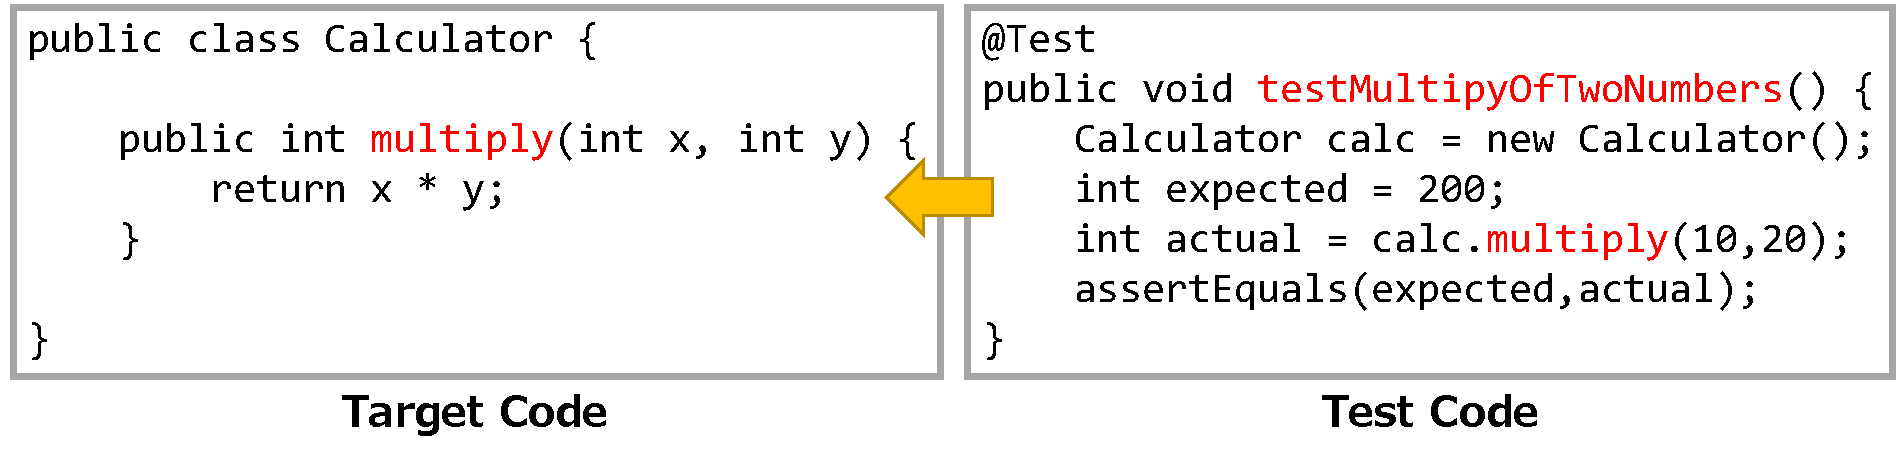
\includegraphics[width=8.5cm]{mapping.pdf}}
\caption{Example of mapping test code to target code.}
\label{fig}
\end{figure}

\begin{enumerate}
\renewcommand{\labelenumi}{(\arabic{enumi})}
\item テストコードを静的解析し,メソッド呼び出しを確認
\item テストメソッドを区切り文字や大文字で分割し,対象メソッドと部分一致した時対応付ける
\end{enumerate}


単体テストでは,図の例のようにテストコード内でオブジェクトの生成が行い,テスト対象コードのメソッド呼び出して実行されます.すなわち,テストコードリポジトリ内のテストコードを静的解析し,メソッド呼び出しを取得することで,テスト対象コードとテストコードを対応付けます.しかし,テストメソッド内では複数のメソッドが呼び出されていることも考えられるのでさらに,メソッド名の比較も行います.テストメソッド名の記述方法としてテスト対象メソッドの処理の内容を忠実に表すことが推奨されており,対象メソッドの名前が記述されていることが多い.したがって,テストメソッドの名前を区切り文字や大文字で分割し,対象メソッドと部分一致した場合,対応付けるように実装した.

図1のテストコードリポジトリには,ソースコードリポジトリ内のプロダクションコードに対応するテストコードが格納されています.我々は,テストコードの検索時間を短縮化するために前処理として事前に大規模なプロジェクトに対して静的解析を行い,プロダクションコードとテストコードの対応付けた情報をDBに保持し,DBを介して高速にテストコードを検索できるようにした.

\subsection{Test Smells Detection}
本研究では,テストスメル検出ツールとしてtsDetect[6]を採用した.tsDetectはASTベースの検出手法で実装されたツールであり,19個のテストスメルを検出できるツールである.また,85%〜100%の精度と90%〜100%の再現率でテストスメルを正しく検出できることが報告されている.本研究では,tsDetectで検出できる19個のテストスメルの内テストコードの推薦を考える上で重要な以下の6種類のテストスメルを提示するように実装しました.

\begin{table}[hbtp]
\caption{Subject Test Smells}
\begin{tabular}{|l|p{5.2cm}|}
\hline
\textbf{Name}                   & \textbf{Description}                                                                                                       \\ \hline
\textbf{Assetion Roulette}        & 1つのテストメソッド内に複数のassert文が存在するテストコード.各assert文は異なる条件をテストするが,テストが失敗した場合開発者へ各assert文のエラーメッセージは提供されないので,失敗を特定することが困難になる.  \\ \hline
\textbf{Conditional Test Logic} &テストメソッド内に複数の制御文が含まれているテストスイート.テスト成功・失敗は制御フロー内にあるassert文に基づくの予測するのが難しい.                                                                                                                                                                                                           \\ \hline
\textbf{Default Test}            &JUnitなどのテスティングフレームワークを使用したテストコードの内,テストクラスやテストメソッドの名前がデフォルトの状態であるテストコード.テストコードの可読性の向上ために適切な名前に変更する必要がある.                                                                                                      \\ \hline
\textbf{Eager Test }             &テスト対象クラス内の複数のメソッドを呼び出しているテストコード.1つのテストメソッド内で複数のメソッド呼び出しを行うと,正確に何をテストしているかについて混乱が生じる.                                                                                                         \\ \hline
\textbf{Exception Handling}      & テストメソッド内で例外処理が含まれているまたは例外を投げるテストコード.例外処理はプロダクションコードに記述し,テストコード内で例外処理が正しく行われるかどうかを確かめるようにリファクタリングする必要がある.                                                                                                    \\ \hline
\textbf{Mystery Guest}          & テストメソッド内で、外部リソースを利用するテストコード.テストメソッド内だけで完結せず外部のファイルなど,外部リソースを利用すると外部との依存関係が生じ,外部リソースが壊れた場合テストも失敗してしまう.                                                                                                                \\ \hline
\end{tabular}
\end{table}


また,前処理として推薦テストコードとしてふさわしくない以下の4つのテストスメルを含むテストコードを事前にテストコードリポジトリから削除し,推薦されるテストコードでとして出力されないようにした. 

\begin{itemize}
\item \textbf{Empty Test.}テストメソッド内にテストの記述はなくコメントのみが含まれているテストコード
\item \textbf{Ignored Test.}@Ignoreアノテーションがあり,実行されないテストコード
\item \textbf{Redundant Assertion.}必ずテストが成功する意味のないテストコード
\item \textbf{Unknow Test.}assertメソッドが存在しないテストコード
\end{itemize}

\subsection{Sort Recommended Test Suites}
入力コードと検出された類似コードの類似度とテストスイート内に含まれるテストスメルの数を基に推薦されるテストスイートの並び替えを行った.我々の以前の調査で,OSS上の有名プロジェクト内の両方のコードフラグメントにテストコードが存在するクローンペアを対象にプロダクションコードとなるクローンペアの類似度とそれに対応するテストコードの類似度を調査した.その結果,テストコードの間の類似度と対象のクローンペアの類似度には相関関係があり,プロダクションコードの類似度が高いほど,テストコード間の類似度も高いことが分かっている.したがって,入力コードと類似コード間の類似度が高いクローンペアほどテストコードの再利用がしやすいと考える.SuiteRecではこの結果を基に類似度が高いクローンの順に並び替えさらに類似度が同じだった場合,テストスメルの数で順番を決めるような推薦ランキングを実装した.

\begin{figure}[htbp]
\centerline{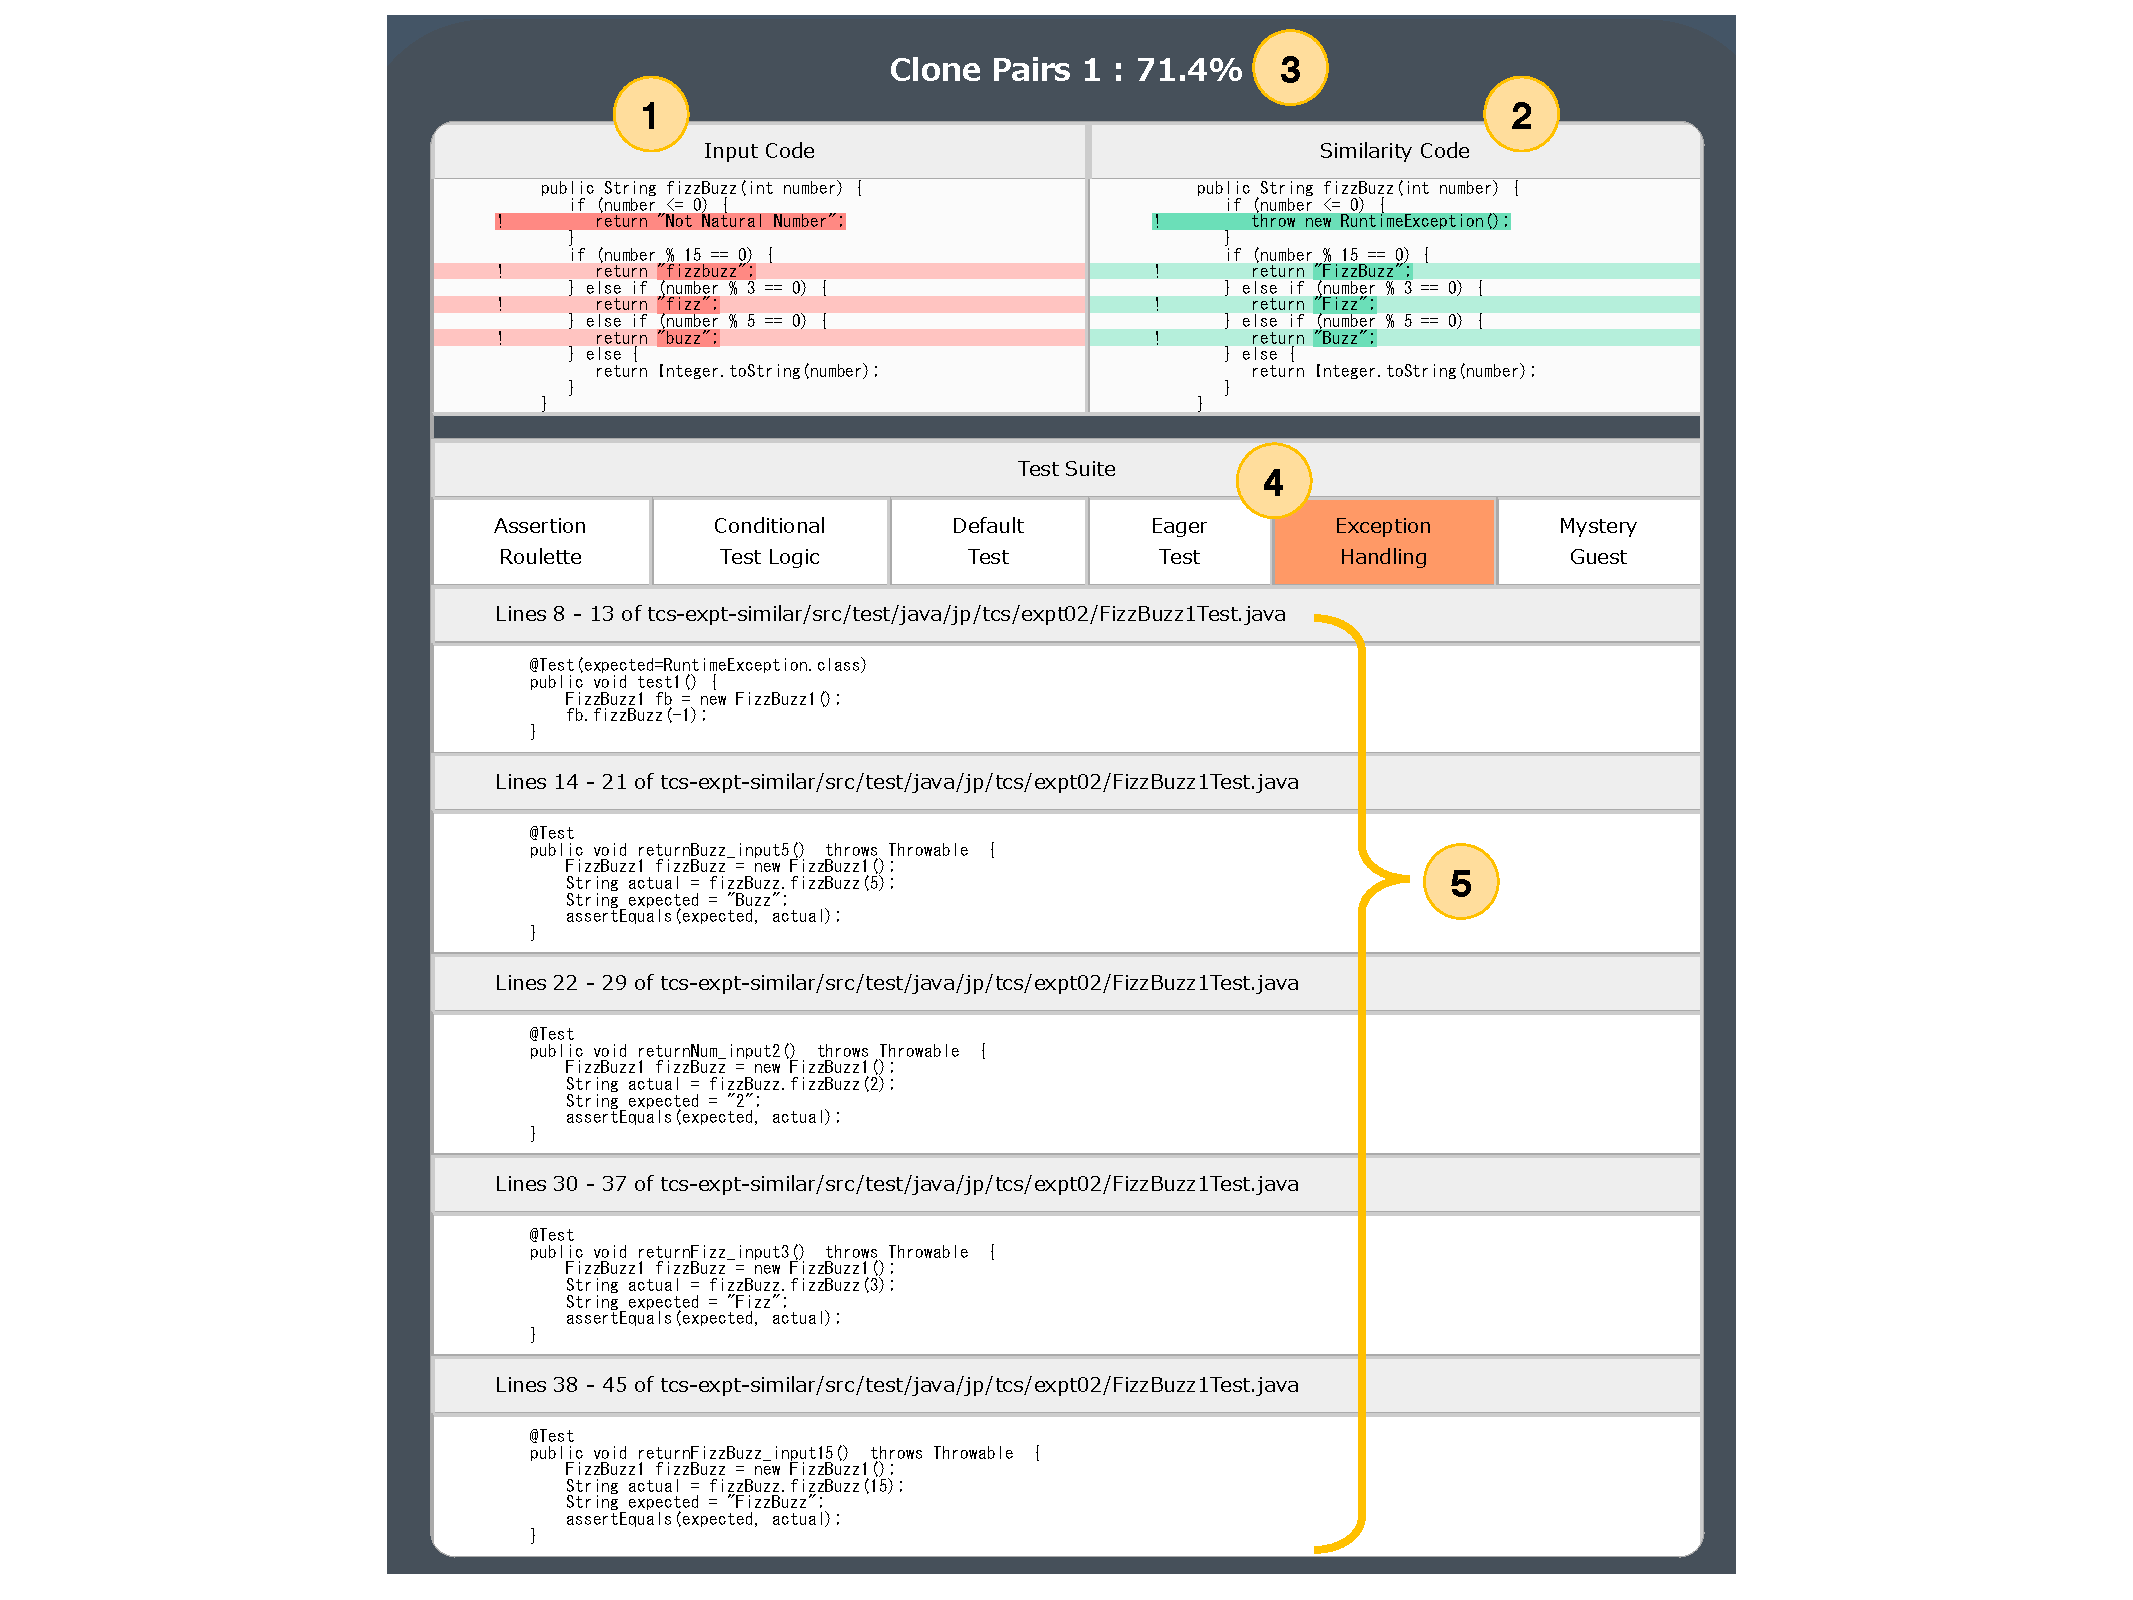
\includegraphics[width=8.7cm]{SuiteRec.pdf}}
\caption{Test suite recommended by SuiteRec.}
\label{fig2}
\end{figure}

 \begin{enumerate}
\renewcommand{\labelenumi}{\textcircled{\scriptsize \theenumi}}
\item{\textbf{Input Code.}開発者が入力した関数単位のプロダクションコードが表示されます.}
\item{\textbf{Similarity Code.}入力コードに対する類似コードが表示されます.入力コードと類似度コードの違いが分かるように差分がハイライトされます.}
\item{\textbf{Degree of similarity.}入力コードと類似コードの類似度が表示されます.類似度はNICADで用いられている計算方法Unique Percentage of Items(UPI)を採用しています.}
\item{\textbf{Test Smells.}推薦されるテストスイート内にテストスメルが含まれている場合,そのテストスメルがオレンジ色にハイライトされ開発者にテストスメルの存在を提示させます.}
\item{\textbf{Recommend Test Suites.}推薦されるテストスイートが表示されます.また,どのプロジェクトからテストコードが参照されたのかを示すためにファイルパスも表示されます.}
\end{enumerate}


\section{Evaluation}

このセクションでは,SuiteRecの定量的及び定性的に評価するために,被験者による実験を行います.被験者は,3つのプロダクションコードのテストコードを作成してもらいます.そしてSuiteRecを使用して作成した場合とそうでない場合のテストコードを比較することで評価を行います.実験を通してコードカバレッジ,実験タスクを終了するまでの時間およびテストコードの品質に関するデータを収集することで,以下のリサーチクエスチョンに答えることを目指します.

\begin{itemize}
\item RQ1 : \textbf{SuiteRecの利用は,開発者の作成したテストコードのカバレッジにどう影響するか?}ソフトウェアの品質を確認する1つの指標としてカバレッジは重要な要素である.テストコード内で一度も実行されない行が存在するとその部分の品質を確保することはできません.SuiteRecの利用は高いカバレッジを達成するために役に立つのでしょうか?
\item RQ2 : \textbf{SuiteRecの利用は,開発者のテストコード作成時間に影響するか?}開発者はSuiteRecで推薦されるテストコードを参考にすることで,テストコード作成時間を短縮化できるのか?
\item RQ3 : \textbf{SuiteRecの利用は,作成したテストコードの品質にどう影響するか?}開発者はSuiteRecで推薦されるテストコードを参考にすることで,品質の高いテストコードを作成することができるのか?
\item RQ4 : \textbf{SuiteRecの利用は,開発者のテストコード作成タスクの認識にどう影響しますか?}SuiteRecを利用した場合,テストコードの作成が容易になり,自分で作成したテストコードに自信が持てるのか?
\end{itemize}

\subsection{Participant Selection}
我々は,基本的なプログラミングスキルを保有し,ソフトウェアテストに理解がある情報系の修士の学生10人対して行った.事前アンケートによると9割以上の学生が2年以上のプログラミング経験があり,8割以上の被験者が1年以上のJava言語の経験があった.また,すべての学生が授業などの講義でソフトウェアテストに関する基本的な知識を持っており,8割以上が単体テストの作成経験があった.

\subsection{Object Selection}
実験を行うために,3つのプロダクションコードを用意した.被験者はテストコードを作成するのでプロダクションコードの仕様を十分理解していることが前提になる.そこで,我々はプロダクションコードとして競技プログラミングをよく用いられる典型的な計算問題を選択した.また,そのプロダクションコードの仕様を確認できるように自然言語で書かれた仕様書を用意した.3つの各問題で違いを出すために問題1,2,3の順に条件分岐の数を8,16,24と多くなるように設定した.図4は,出題したプロダクションコードの一例である.実験後のアンケートで,実験タスクについての理解を確認したがすべての被験者が実験タスクの理解についてポジティブな意見を述べたことが分かっている.また,十分な実験時間があったかどうかに関する質問に対してもネガティブな回答はなかった.したがって,被験者は与えられた実験タスクに対して十分に理解し,作業時間も十分にあったことが分かる.

\begin{figure}[htbp]
\centerline{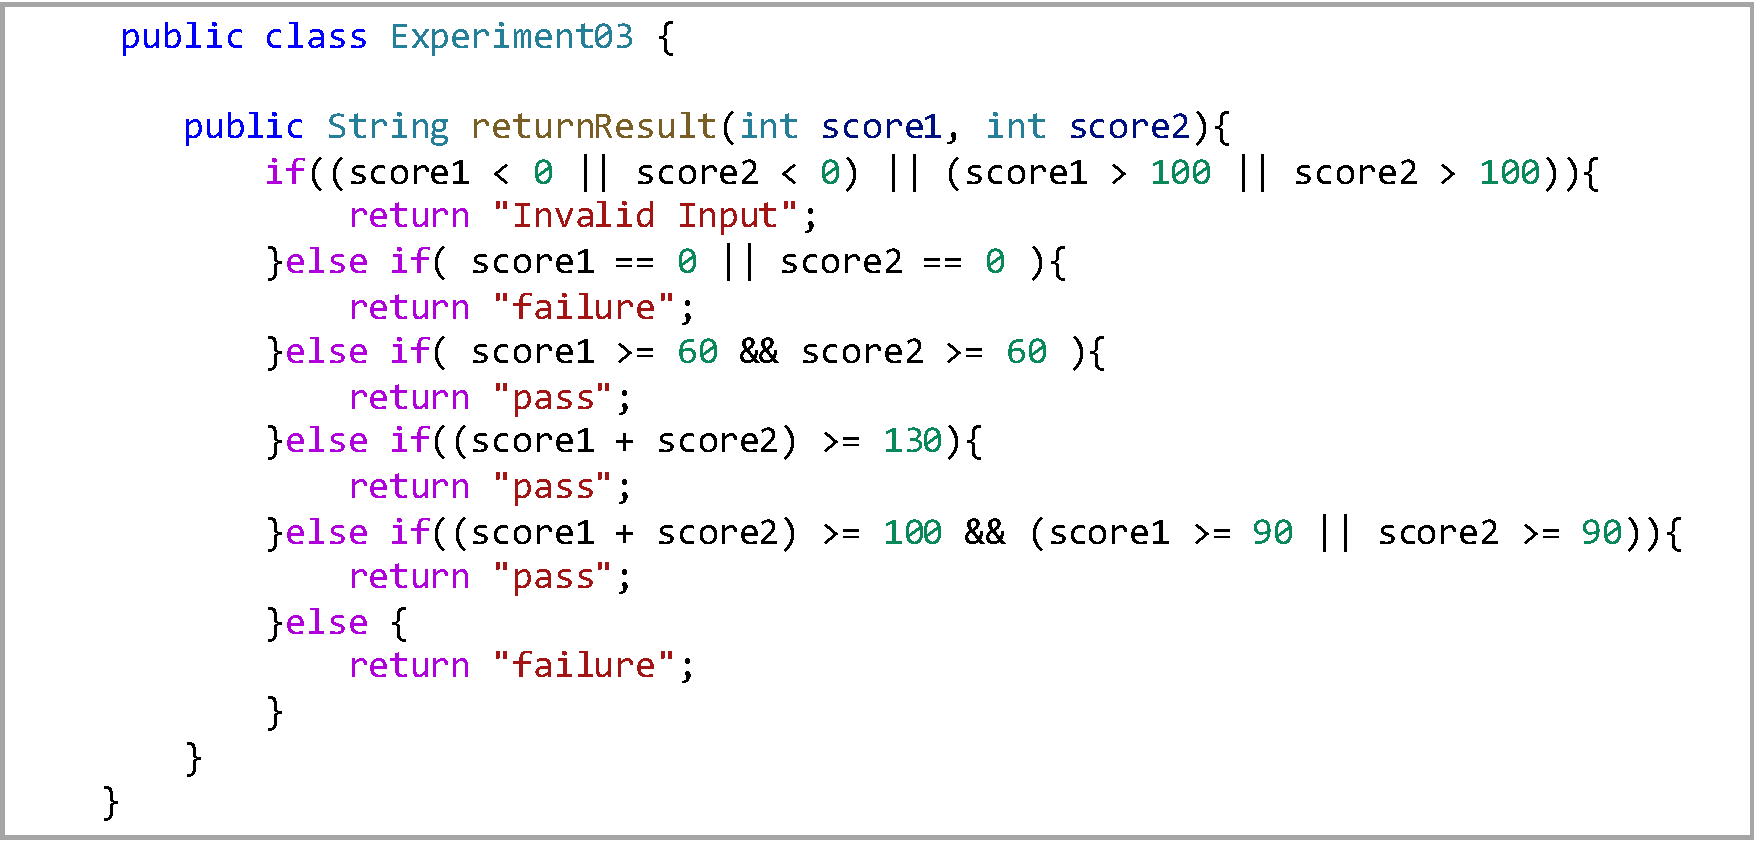
\includegraphics[width=8.5cm]{task.pdf}}
\caption{Example of a experimental task.}
\label{fig3}
\end{figure}

\subsection{Experiment Procedure}
まず初めにソフトウェアテストに関する基本的な知識からJUnitを使用に関する30分の講義と練習問題を実施し,テストコードの記述に対する理解を確認した.そして本番の実験課題の3つのプロダクションコードのテストコードを作成してもらった.実験タスクの終了は被験者に判断してもらう.具体的には,被験者自身が作成したテストコードのカバレッジ・品質に満足した時,実験タスクを終了してもらった.実験時間は1問につき最大25分の時間を設けた.推薦ツールの利用効果が問題によって偏らないように,被験者によってツールを利用の有無を問題によって変えるように割り当てた.また,推薦ツールを利用した場合の学習効果を防ぐために,3つの問題で連続してツールを利用しないようにタスクの割り当てを行った.また,過去の回答を参考にできないようにした.

\section{Results}

このセクションでは,10人の被験者によるSuiteRecの定量的および定性的評価結果を報告する.前のセクションで説明したように,4つの研究課題について分析結果を提示します.

\subsection{RQ1: SuiteRecの利用は,開発者の作成したテストコードのカバレッジにどう影響するか?}
本実験では,被験者によって提出されたテストスイートの命令網羅と分岐網羅の2種類のコードカバレッジの計算した.カバレッジの計算には統合開発環境Eclipseのプラグインとして搭載されているEclEmmaを利用した.図1と図2はそれぞれ被験者による命令網羅と分岐網羅の平均カバレッジを示す.結果として,命令網羅の割合は3つの問題すべてにおいてツールを利用した場合とそうでない場合で網羅率にほとんど違いはなく,どの問題も網羅率が90\%を超えている.図2の分岐網羅についても分岐数が少ないTASK1とTASK2についてはツールを使用した場合とそうでない場合でほとんど差がないことが分かる.しかし,プロダクションコードの分岐数が最も多いTASK3については,実験者の平均カバレッジに10\%以上の差があることが分かった.この結果は,分岐が多いプロダクションコードのテストコードを作成する際に,SuiteRecで推薦されるテストコードは網羅率を向上するのに役に立つことが考えられる.実際に実験後のアンケートの記述欄には,推薦コードによって見落としていたテスト項目をフォローすることができたという報告が複数存在した.
\begin{figure}[htbp]
\centerline{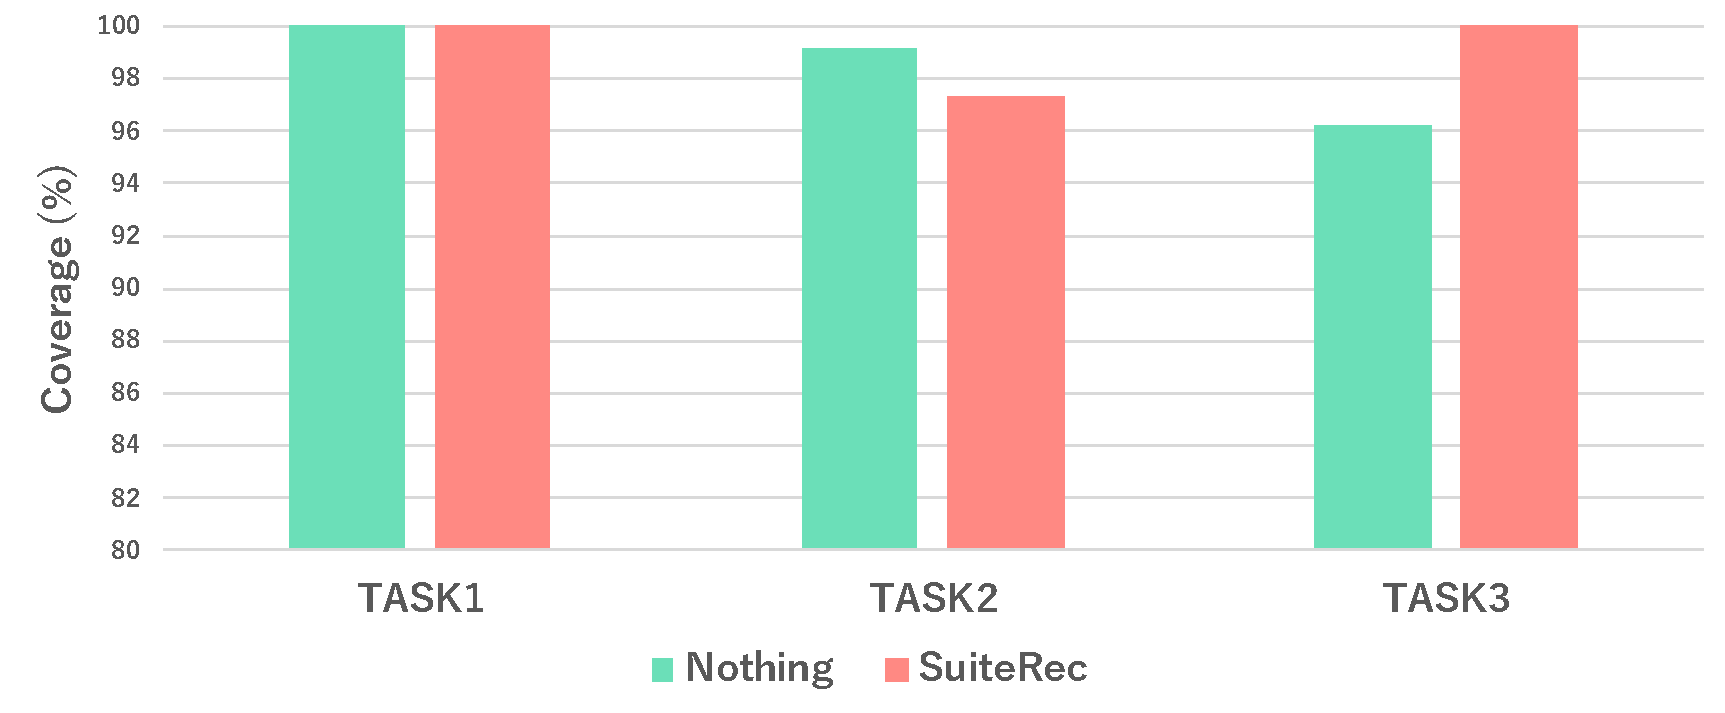
\includegraphics[width=8.5cm]{C0.pdf}}
\caption{Statement coverage (C0).}
\label{fig4}
\end{figure}

\begin{figure}[htbp]
\centerline{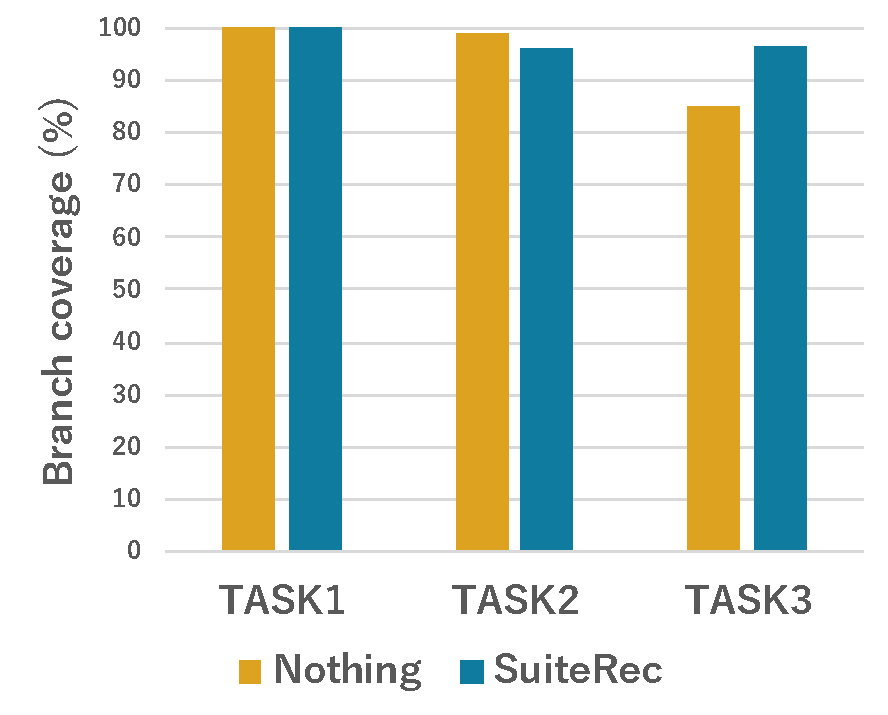
\includegraphics[width=8.5cm]{C1.pdf}}
\caption{Branch coverage (C1).}
\label{fig5}
\end{figure}

\subsection{RQ2: SuiteRecの利用は,開発者のテストコード作成時間に影響するか?}

図5は,SuiteRecを使用した場合と何も使用しない場合で,テストコード作成タスクの終了までに費やされた時間を比較しています.3つの問題の内,2つの問題でSuiteRecを使用した場合そうでない場合と比べてテスト作成時間が大きくなっていることが分かる.この結果はSuiteRecによって推薦される複数のテストスイートを読み理解するのに時間がかかる可能性があります.被験者は,推薦されるテストコードをそのままの形で再利用することができません.入力したプロダクションコードと検出された類似コードの差分を見てテストコードを書き換える必要があります.また,実験後のアンケートではテスト対象のオブジェクト生成の記述を再利用する際にその都度書き換える必要があり,時間がかかってしまったと述べている.問題2については,SuiteRecを利用した場合の方がテスト作成時間が短いことが分かる.我々は,提出されたテストコード調査したところカバレッジに差はないもののSuiteRecを使用しない場合はテストケース(項目)の数多くなっていることが分かった.この結果は,被験者は無駄なテストケースを多く記述するのに無駄な時間を費やしてしまった可能性がある.
\begin{figure}[htbp]
\centerline{\includegraphics[width=8.5cm]{duration.pdf}}
\caption{Time taken to create test code.}
\label{fig6}
\end{figure}

\subsection{RQ3 : SuiteRecの利用は,作成したテストコードの品質にどう影響するか?}

図6はSuiteRecを使用した場合とそうでない場合で,提出されたテストコード内のテストスメル数を比較しています.すべてのTASKに対して,SuiteRecを使用して作成されたテストコードはテストスメルをあまり含んでいないことが分かる.この結果は,推薦されるテストコード自体の品質が高く開発者はそれを再利用することで品質を維持したままテストコードを作成したと考えられる.また,ツールの出力画面で推薦されるテストスイート内に含まれているテストスメルを提示することで,それを基にテストコードを書き替えより品質が高いテストコードを提出した可能性が考えられる.実際のアンケートの記述でも提示されたテストスメルを理解し,それをなくすようにリファクタリングしテストコードを作成したという報告がされている.一方で,テストスメルが含まれていることは気づいていたがリファクタリングの方法が分からずそのまま提出したと述べている被験者も存在した.これは今後のツールの課題であり,テストスメルのリファクタリング方法も提示する改良の必要がある.SuiteRecを使用しなかった場合は,使用した場合と比べ全体として5倍以上の被験者はテストスメルを埋め込んでいた.その中でも多く埋め込まれていたテストスメルとして,Assertion Roulette, Default Test, Eager Testが挙げられる.多くの被験者は,初期状態のテストメソッドの名前を変更せず一つのテストメソッド内でコピーアンドペーストによってAssert文を記述していたのが原因だと考えられる.実際に既存研究でもこれらのテストスメルが既存プロジェクトで多く検出されていることが報告されている[6]. 

\begin{figure}[htbp]
\centerline{\includegraphics[width=8.5cm]{smells.pdf}}
\caption{Number of detected test smells.}
\label{fig7}
\end{figure}

\begin{figure*}[t]
 \begin{center}
  \includegraphics[width=18.5cm]{suiterec-expt.pdf}
  \caption{キャプション}
  \label{}
 \end{center}
\end{figure*}

\subsection{RQ4 : SuiteRecの利用は,開発者のテストコード作成タスクの認識にどう影響しますか?}

図7は,実験後のアンケートの回答の結果をまとめたものです.初めの2つの質問から,被験者は,実験タスクを明確に理解し(質問1),実験タスクを終えるのに十分な時間があったことが分かる(質問2).残りの質問については,SuiteRecを使用した場合とそうでない場合で,実験タスクに対する意見に違いがあることが分かります.

被験者はテストコードを作成する際に,SuiteRecを用いるとテストコード作成を容易に感じることができます.しかし,この結果はこの結果は実際のタスクの終了時間と長さ(図2)とは対照的であり,SuiteRecを使用した場合の方がタスクの終了時間が遅いことが分かります.被験者は,推薦された複数提案されるテストスイートを読み理解して再利用するかどうかを決定します.また,テストコードはそのままの状態で適用することはできず,入力コードと検出された類似コードの差分を理解しテストコードに適切な修正を加える必要があります.我々は,SuiteRecを使用した場合被験者はこの部分に多くの時間を費やすことがあると推測しています.アンケートによるツールの改善点への自由記述では,テストコードの編集作業を支援する機能(クラス名やメソッド名を入力コード対応する名前に自動編集する機能など)を追加した方が良いという多くの意見を頂来ました.SuiteRecの更なる改善は,実験タスクの完了時間を短縮できる可能性を示しています.

被験者は,SuiteRecを使用した場合,自身で作成したテストコードのカバレッジに自信があることが分かる(質問5).一方で,何も使用しなかった場合40\%の被験者がネガティブな回答を報告している.しかし,実際に提出されたテストコードのカバレッジにはほとんど差がないことが分かっています(図3).自身が作成したテストコードのカバレッジに自信を持つことは重要です.開発者は,自分の書いたコードに責任を持ち,不安なくソフトウェアをユーザに提供できることは,ソフトウェアテストを行う目的の一つです.

被験者は,何も使わずテストコードを作成した場合40\%の被験者が自身の書いたテストコードの品質に自信が持てません.実際の提出されたテストコード内のテストスメルの数もSuiteRecを使わなかった場合は,使った場合と比べて多く存在していることが分かります(図4).開発者は無意識の内にテストスメルを埋め込みそれが後のメンテナンス活動を困難にさせます.SuiteRecの利用は,開発者にテストコードの品質に対する意識を与えることでテストメルの数を減らし,作成したコードに自信をもたらします.一方で,SuiteRecを利用した場合でも品質に関してネガティブな意見も存在します.アンケートの記述項目では,テストスメルの存在は意識できたが具体的にどう修正してなくすことができるのか分からなかったと報告されています.これはSuiteRecの更なる改善の必要性を示しており,各テストスメルに対するリファクタリング方法も提示する機能を追加すべきだと考えている.

\section{Related work}
\textbf{Code recommendation.}コード推薦システムは,他のプログラムのコードフラグメントを提示し再利用できるようにしたりすることで開発者を支援します.Zhang[1]らはクローンペア間で,コードを移植を行い移植前と移植後のテスト結果を比較しその情報を基にテストを再利用する手法を提案している.Mostafa[2]らは,自身のプロジェクトだけでなく他のプロジェクトを横断してクローンペアを検出しテストコード再利用することの有効性を調査した.

\section{Conclusion and Future Work}

SuiteRecは,ユーザーが入力した関数単位のプロダクションコードに対して,類似コード検出ツールを用いてOSS上に存在する既存のテストコードを推薦するツールです.さらに,テストコードの良くない実装を表すメトリクスであるテストスメルを開発者に提示し,より品質の高いテストスイートを推薦できるように推薦順位がランキングされています.分岐が多くテスト項目の作成が難しいプロダクションコードに対して,SuiteRecを使用してテストコード作成するとカバレッジを向上できる可能性があります.また,品質の高いテストコードを作成でき,開発者は自分で書いたコードに自信が持つことができます.今後の課題としては,より実践的な利用に備えてツールを改善する必要があります.さらにSuiteRecが推薦するテストスイートの優先順位に対する妥当性評価も実施する予定である.


\begin{thebibliography}{15}
\bibitem{b1} S. Shamshiri, J. M. Rojas, and J. P. Galeotti, ``How Do Automatically Generated Unit Tests Influence Software Maintenance?," In {\it Proceedings of the International Conference on Software Testing, Verification and Validation (ICST)}, pp.239--249, 2018. 

\bibitem{b2} C. K. Roy and J. R. Cordy, ``NICAD: Accurate Detection of Near-Miss Intentional Clones Using Flexible Pretty-Printing and Code Normalization," In {\it Proceedings of the International Conference on Program Comprehension (ICPC)}, pp.172--181, 2008.

\bibitem{b3} G. Fraser and A. Arcuri, ``EvoSuite: automatic test suite generation for object-oriented software," in  {\it Proceedings of the Symposium on the Foundations of Software Engineering (FSE)}, pp. 416--419, 2011.

\bibitem{b4} N. Koochakzadeh and V. Garousi, ``Tecrevis: a tool for test coverage and test redundancyvisualization," Testing–Practice and Research Techniques, 2010.

\bibitem{b5} M.Greiler, A.Zaidman, A.v.Deursen, and M.-A.Storey, ``Strategies for avoiding text fixture smells during software evolution," In {\it Proceedings of the 10th Working Conference on Mining Software Repositories (MSR)}, pp. 387--396, 2013.

\bibitem{b6} G. Meszaros. xUnit Test Patterns: Refactoring Test Code. Addison Wesley, 2007.

\bibitem{b7} A. van Deursen, L. Moonen, A. Bergh, and G. Kok. Refactoring test code. In {\it Proceedings of the 2nd International Conference on Extreme Programming and Flexible Processes in Software Engineering (XP)}, pp. 92--95, 2001.

\bibitem{b8} D. Spadini, F. Palomba, A. Zaiaman, M. Bruntink, and A.Bacchelli, ``On The Relation of Test Smells to Software Code Quality," In {\it Proceedings of the International Conference on Software Maintenance and Evolution (ICSME)}, pp. 1--12, 2018. 

\bibitem{b9} A. Peruma, K. Almalki, C. D. Newman, M. W. Mkaouer, A. Ouni, and F. Palomba, ``On the Distribution of Test Smells in Open Source Android Applications: An Exploratory Study," In {\it Proceedings of the International Conference on Computer Science and Software Engineering (CASCON)}, pp. 193--202, 2019.

\bibitem{b10} S. U. T. Smells. http://testsmells.github.io/, 2018.

\bibitem{b11} https://www.eclemma.org/

\bibitem{b21} https://www.eclipse.org/

\bibitem{b12} P. Machado and A. Sampaio, ``Automatic Test-Case Generation," Testing Techniques in Software Eng., vol. 6153, pp. 59--103, 2010. 

\bibitem{b13} S. Panichella, A. Panichella, M. Beller, A. Zaidman, and H. C. Gall, ``The impact of test case summaries on bug fixing performance: An empirical investigation," In {\it Proceedings of the International Conference on Software Engineering (ICSE)}, pp. 547--558, 2016.

\bibitem{b14} E. Daka, J. Campos, G. Fraser, J. Dorn, and W. Weimer, ``Modeling readability to improve unit tests," In {\it Proceedings of the Joint Meeting on Foundations of Software Engineering (ESEC/FSE)}, pp. 107--118, 2015.

\bibitem{b15} F. Palomba, A. Panichella, A. Zaidman, R. Oliveto, and A. De Lucia, ``Automatic test case generation: what if test code quality matters?," In {\it Proceedings of the International Symposium on Software Testing and Analysis (ISSTA)}, pp. 130--141, 2016.

\bibitem{b16} L. Ma, C. Artho, C. Zhang, H. Sato, J. Gmeiner, and R. Ramler. ``Grt: Program-analysis-guided random testing (t)," In {\it Proceedings of the International Conference on Automated Software Engineering (ASE)}, pp. 212--223, 2015.

\bibitem{b17} A. Panichella, F. Kifetew, and P. Tonella. ``Reformulating branch coverage as a many-objective optimization problem," In {\it Proceedings of the International Conference on Software Testing, Verification and Validation (ICST)}, pp. 1--10, 2015. 

\bibitem{b18} I. W. B. Prasetya. ``T3, a Combinator-Based Random Testing Tool for Java: Benchmarking," In {\it International Workshop on Future Internet Testing}, pp. 101--110. Springer, 2014.

\bibitem{b19} A. Sakti, G. Pesant, and Y.-G. Gu\'{e}h\'{e}neuc. ``Instance Generator and Problem Representation to Improve Object Oriented Code Coverage," {\it Transactions on Software Engineering}, pp. 294--313, 2015.

\bibitem{b20} M. Ellims, J. Bridges, and D. C. Ince, ``The economics of unit testing," Empir. Softw. Eng., vol. 11, no. 1, pp. 5--31, 2006.

\bibitem{b22} F. Appel. Testing with JUnit. Packt, 2015.

\end{thebibliography}

\begin{comment}
\vspace{12pt}
\color{red}
IEEE conference templates contain guidance text for composing and formatting conference papers. Please ensure that all template text is removed from your conference paper prior to submission to the conference. Failure to remove the template text from your paper may result in your paper not being published.
\end{comment}
\end{document}
